% !TEX TS-program = lualatex
\documentclass[11pt,a4paper]{article}

\newcommand{\DocID}{IFOG-VPROTO-ARCH-001}
\newcommand{\DocVersion}{v2.0.0}
\newcommand{\DocDate}{2026-11-25}

\usepackage{fontspec}
\setmainfont{Noto Sans}
\setmonofont{DejaVu Sans Mono}[Scale=0.84]

\usepackage[a4paper,margin=2.0cm,headheight=14pt]{geometry}
\usepackage{amsmath,amssymb}
\usepackage{booktabs,longtable,tabularx,array}
\usepackage[htt]{hyphenat}
\usepackage{graphicx}
\usepackage{xcolor}
\usepackage{tikz}
\usetikzlibrary{arrows.meta,positioning,fit,shapes.geometric,backgrounds}
\usepackage{tcolorbox}
\usepackage{fancyhdr}
\usepackage{hyperref}

\definecolor{NavyBlue}{HTML}{1B365D}
\definecolor{TealDark}{HTML}{0E6251}
\definecolor{SlateBg}{HTML}{F4F7FA}
\definecolor{BorderGray}{HTML}{CBD5E0}
\definecolor{Crimson}{HTML}{9B2C2C}

\hypersetup{
    colorlinks=true,
    linkcolor=NavyBlue,
    urlcolor=TealDark,
    pdftitle={IFOG Virtual Prototype System Architecture (\DocVersion)},
    pdfauthor={Duy-Huan / ifog-vproto}
}

\pagestyle{fancy}
\fancyhf{}
\fancyhead[L]{\small\color{NavyBlue}\textbf{\DocID} --- IFOG Virtual Prototype Architecture}
\fancyhead[R]{\small\color{TealDark}\textbf{\DocVersion} (\DocDate)}
\fancyfoot[C]{\small\thepage}
\renewcommand{\headrulewidth}{0.5pt}

\setlength{\parskip}{0.42em}
\setlength{\parindent}{0pt}
\sloppy
\emergencystretch=3em

\begin{document}

% --- Title Banner ---
\begin{tcolorbox}[colback=NavyBlue,colframe=NavyBlue,arc=4pt,boxrule=0pt,left=12pt,right=12pt,top=10pt,bottom=10pt]
{\color{white}\Large\bfseries Closed-Loop IFOG Multi-Scale Virtual Prototype}\\[4pt]
{\color{white}\large System Architecture \& Implementation Specification}\\[6pt]
{\color{white}\small Document ID: \texttt{\DocID} \quad|\quad Version: \texttt{\DocVersion} \quad|\quad Normative Spec: \texttt{IFOG-SIM-SPEC-005} v5.0 / \texttt{SPEC-004} v4.0 \quad|\quad Date: \DocDate}
\end{tcolorbox}

\section{Document Control \& Revision History}

\small
\begin{tabularx}{\textwidth}{@{}p{3.6cm} X@{}}
\toprule
\textbf{Document Field} & \textbf{Controlled Value} \\
\midrule
Document Identifier & \texttt{\DocID} \\
Current Version & \texttt{\DocVersion} (Synchronized with \texttt{pyproject.toml} per \texttt{AGENT.md} Rule 16) \\
Release Status & \textcolor{TealDark}{\textbf{RELEASED --- Production CI/CD, 41-Formula \& 5-Gate + 11-Scenario Verified}} \\
Normative Authority & \texttt{spec/IFOG-SIM-SPEC-005.tex} (v5.0) \& \texttt{spec/IFOG-SIM-SPEC-004.tex} (v4.0) (both SHA-256 locked) \\
Scenarios Companion & \texttt{docs/IFOG\_SIMULATION\_SCENARIOS.\{md,tex,pdf\}} (\DocVersion) \\
Reference Standards & IEEE Std 952-2020 (IFOG Test \& AVAR); IEEE Std 1666.1-2016 (SystemC-AMS) \\
Markdown Companion & \texttt{docs/IFOG\_VPROTO\_ARCHITECTURE.md} \\
\bottomrule
\end{tabularx}

\vspace{0.5em}
\begin{tabularx}{\textwidth}{@{}p{1.4cm} p{2.0cm} p{3.2cm} X@{}}
\toprule
\textbf{Version} & \textbf{Date} & \textbf{Milestone} & \textbf{Summary of Architectural Changes} \\
\midrule
\texttt{v1.0.0} & 2026-11-25 & Initial Full Release & Complete 3-Tier Virtual Prototype (\texttt{tier1\_offline}, C++17 SystemC-AMS 2.3.4 \texttt{tier2\_sysc\_ams}, \texttt{tier3\_analysis}, \texttt{viz}), 30/30 formula verification, 100\% C++ \& Python coverage, real 4-Gate acceptance suite, strict 2-branch CI/CD. \\
\texttt{v1.1.0} & 2026-11-25 & Auto-Reporting \& Doc-Sync & Added automatic \texttt{.md} + interactive \texttt{.html} reporting and dashboard index under \texttt{report/}; unified simulation runner (\texttt{scripts/run\_sim.sh}, \texttt{scripts/run\_sim.py}, \texttt{sim\_runner\_cli.py}); full release docs (\texttt{.md}/\texttt{.tex}/\texttt{.pdf}) under \texttt{docs/}; enacted \textbf{Rule 16} mandatory version--document sync CI gate. \\
\texttt{v1.2.0} & 2026-11-25 & Portable Containers \& Example & Added universal Git-source installers for SystemC 2.3.4, SystemC-AMS 2.3.4, \texttt{nlohmann/json}, and Python venv (\texttt{scripts/setup\_env.sh}, \texttt{scripts/env.sh}); added Docker/Podman suite (\texttt{Containerfile}, \texttt{Dockerfile}, \texttt{compose.yaml}, \texttt{scripts/container\_run.sh}); executed and committed full real 4-Gate feasibility example (\texttt{examples/full\_4gate\_baseline/}). \\
\texttt{v2.0.0} & 2026-11-25 & \texttt{SPEC-005} 6-State DSP \& 11 Scenarios & Upgraded normative spec to \texttt{IFOG-SIM-SPEC-005} v5.0 (41/41 formulas \texttt{EQ-01}--\texttt{EQ-41}); implemented official 6-state symmetric DSP ($+136.94\text{ dB}$ RAM/xtalk rejection, $-33.3\%$ $V_{\text{peak}}$), 64 B \texttt{dsp\_trace.bin}, real-time FPGA BIT/FDIR, ADC aperture jitter, VRE/Faraday, concurrent 3-axis SystemC-AMS IMU (\texttt{--imu3axis}), 6 Time-Domain + 5 Engineering scenarios (\texttt{scripts/run\_all\_scenarios.sh}, 22 CLI modes), and \texttt{docs/IFOG\_SIMULATION\_SCENARIOS.\{md,tex,pdf\}}. \\
\bottomrule
\end{tabularx}
\normalsize

\vspace{0.5em}
\tableofcontents
\newpage

\section{System Context \& Multi-Scale Architecture}

\texttt{ifog-vproto} implements a deterministic, high-fidelity virtual prototype of a \textbf{Closed-Loop Interferometric Fiber-Optic Gyroscope (IFOG)} supporting both 2-state and 4-state Lef\`evre phase modulation. The simulator resolves 11 orders of magnitude in temporal dynamic range---from sub-microsecond electro-optic TIA/MIOC transient dynamics ($\Delta t_{\text{fast}} = \tau / K \approx 306\text{ ns}$) to 10-hour IEEE Std 952 Overlapping Allan Variance curves ($3.6\times 10^6$ samples at $100\text{ Hz}$)---while maintaining 64-bit IEEE-754 phase precision ($< 10^{-15}\text{ rad}$ modulo-$2\pi$ wrapping error).

\begin{figure}[h!]
\centering
\resizebox{\textwidth}{!}{%
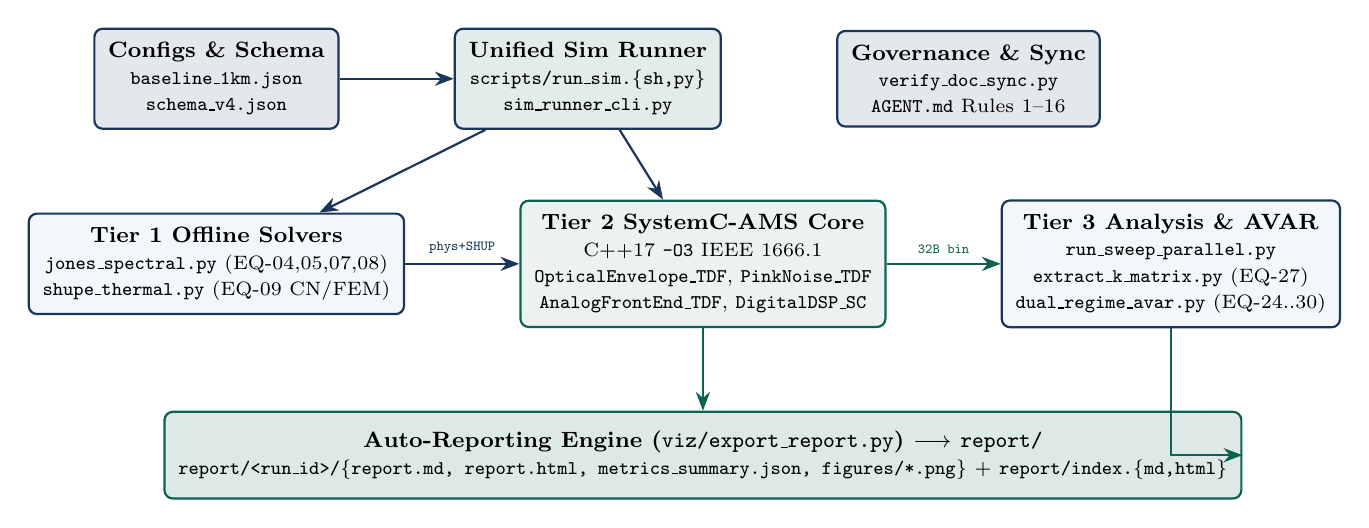
\begin{tikzpicture}[
    node distance=0.95cm and 1.35cm,
    box/.style={rectangle,rounded corners=3pt,draw=NavyBlue,fill=SlateBg,thick,align=center,font=\footnotesize,minimum width=3.1cm,minimum height=1.1cm,inner sep=5pt},
    arr/.style={-{Stealth[length=2.4mm]},thick,NavyBlue},
    tarr/.style={-{Stealth[length=2.4mm]},thick,TealDark}
]
% Top Runner & Config
\node[box,fill=NavyBlue!12] (cfg) {\textbf{Configs \& Schema}\\{\scriptsize\texttt{baseline\_1km.json}}\\{\scriptsize\texttt{schema\_v4.json}}};
\node[box,fill=TealDark!12,right=1.45cm of cfg] (runner) {\textbf{Unified Sim Runner}\\{\scriptsize\texttt{scripts/run\_sim.\{sh,py\}}}\\{\scriptsize\texttt{sim\_runner\_cli.py}}};
\node[box,fill=NavyBlue!12,right=1.45cm of runner] (docsync) {\textbf{Governance \& Sync}\\{\scriptsize\texttt{verify\_doc\_sync.py}}\\{\scriptsize\texttt{AGENT.md} Rules 1--16}};

% Tier 1
\node[box,below=1.05cm of cfg] (t1) {\textbf{Tier 1 Offline Solvers}\\{\scriptsize\texttt{jones\_spectral.py} (EQ-04,05,07,08)}\\{\scriptsize\texttt{shupe\_thermal.py} (EQ-09 CN/FEM)}};

% Tier 2
\node[box,draw=TealDark,fill=TealDark!8,right=1.45cm of t1,minimum width=3.8cm] (t2) {\textbf{Tier 2 SystemC-AMS Core}\\{\scriptsize C++17 \texttt{-O3} IEEE 1666.1}\\{\scriptsize\texttt{OpticalEnvelope\_TDF}, \texttt{PinkNoise\_TDF}}\\{\scriptsize\texttt{AnalogFrontEnd\_TDF}, \texttt{DigitalDSP\_SC}}};

% Tier 3
\node[box,right=1.45cm of t2] (t3) {\textbf{Tier 3 Analysis \& AVAR}\\{\scriptsize\texttt{run\_sweep\_parallel.py}}\\{\scriptsize\texttt{extract\_k\_matrix.py} (EQ-27)}\\{\scriptsize\texttt{dual\_regime\_avar.py} (EQ-24..30)}};

% Reporting
\node[box,fill=TealDark!14,draw=TealDark,below=1.05cm of t2,minimum width=8.2cm] (rep) {\textbf{Auto-Reporting Engine (\texttt{viz/export\_report.py}) $\longrightarrow$ \texttt{report/}}\\{\scriptsize\texttt{report/<run\_id>/\{report.md, report.html, metrics\_summary.json, figures/*.png\}} + \texttt{report/index.\{md,html\}}}};

\draw[arr] (cfg) -- (runner);
\draw[arr] (runner) -- (t1);
\draw[arr] (runner) -- (t2);
\draw[arr] (t1) -- node[above,font=\tiny]{\texttt{phys+SHUP}} (t2);
\draw[tarr] (t2) -- node[above,font=\tiny]{\texttt{32B bin}} (t3);
\draw[tarr] (t3) |- (rep);
\draw[tarr] (t2) -- (rep);
\end{tikzpicture}%
}
\caption{3-Tier Hybrid Multi-Scale Co-Simulation, Unified Runner, and Automatic Reporting Architecture.}
\end{figure}

\footnotesize
\begin{tabularx}{\textwidth}{@{}p{1.65cm} p{3.1cm} p{4.15cm} X@{}}
\toprule
\textbf{Tier} & \textbf{Engine} & \textbf{Time Scale} & \textbf{Primary Outputs} \\
\midrule
Tier 1 & Python / NumPy / SciPy & Spectral ($N_{\text{spec}}=64..128$) \& Thermal ($0..10\text{ h}$) & \texttt{phys\_params.json}, \texttt{shupe\_lut.bin} (\texttt{SHUP}) \\
Tier 2 & C++17 / SystemC-AMS 2.3.4 & $\Delta t_{\text{fast}} \approx 306\text{ ns}$, $\tau \approx 4.89\ \mu\text{s}$, $0.025..60\text{ s}$ & \texttt{sim\_out.bin} (32 B), \texttt{micro\_waveforms.bin} (64 B), \texttt{sim\_summary.json} \\
Tier 3 & Python / Multiprocessing & $\Delta t_{\text{slow}} = 10\text{ ms}$ ($100\text{ Hz}$), $10\text{ h}$ ($3.6\times 10^6$ pts) & \texttt{sweep\_results.json}, \texttt{k\_matrix.json}, \texttt{avar\_curve.npz}, \texttt{avar\_metrics.json} \\
Viz / Report & Matplotlib + Plotly HTML5 & Automatic post-run & \texttt{report/<run\_id>/\{report.md, report.html, figures/*.png\}} + \texttt{report/index.\{md,html\}} \\
\bottomrule
\end{tabularx}
\normalsize

\section{Tier 1: Offline Optical \& Thermal Solvers}

\begin{itemize}
    \item \textbf{Schema \& Fail-Closed Validation (\texttt{tier1\_offline/config\_loader.py}, \texttt{configs/schema\_v4.json}):} Validates all 13 configuration blocks against JSON Schema Draft 2020-12 and enforces blanking indices $0 \le k_{\text{start}} \le k_{\text{end}} < K$, ADC rails $V_{\min} < V_{\max}$, Jury stability $0 < K_{\text{tot},1} < 1$, and Loop-2 bandwidth separation $K_{\text{tot},2} \le 0.1 K_{\text{tot},1}$ (Rule 11).
    \item \textbf{Spectral-Sliced Jones Matrix Solver (\texttt{tier1\_offline/jones\_spectral.py}):} Evaluates vectorized \texttt{complex128} Jones chains across $M$ PM fiber segments with frequency-proportional birefringence $\Delta\beta(\omega_k) = \frac{2\pi}{L_B}\frac{\omega_k}{\bar{\omega}}$ and strict Lorentz reciprocity $\mathbf{J}_{\text{CCW}}(\omega_k) = \mathbf{J}_{\text{CW}}^T(\omega_k)$ (\texttt{EQ-04}). Computes exact closed-form fringe visibility $V$, polarization bias phase $\phi_{\text{pol}}$ (\texttt{EQ-05}), Sagnac scale factor $K_{\text{opt}}$ (\texttt{EQ-07}), and coherence-weighted Kerr bias $\Delta\phi_{\text{Kerr}}$ (\texttt{EQ-08}).
    \item \textbf{Thermal Shupe Solver (\texttt{tier1\_offline/shupe\_thermal.py}):} Integrates \texttt{EQ-09} with quadrupolar winding asymmetry $\delta z_{\text{quad}}$ from either an unconditionally stable 1D Crank--Nicolson radial diffusion solver (\texttt{scipy.linalg.solve\_banded}) or an external FEM CSV table, emitting the fail-closed binary LUT \texttt{shupe\_lut.bin} (24-byte header \texttt{<4sIQd} with magic \texttt{"SHUP"} followed by \texttt{<dd} pairs).
\end{itemize}

\section{Tier 2: IEEE Std 1666.1 SystemC / SystemC-AMS Closed-Loop Core}

Tier 2 is compiled in C++17 (\texttt{SC\_CPLUSPLUS=201703L}) against Ubuntu 24.04 SystemC 2.3.4 and SystemC-AMS PoC 2.3.4 (pinned commit \texttt{a72d365f}) into static library \texttt{libifog\_core.a}, simulator binary \texttt{build/ifog\_sim}, and test binary \texttt{build/ifog\_cpp\_tests}.

\begin{figure}[h!]
\centering
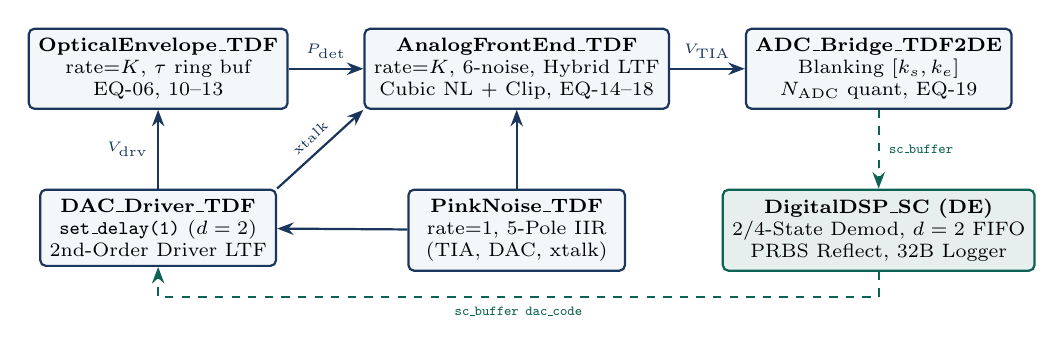
\begin{tikzpicture}[
    node distance=0.75cm and 0.85cm,
    tdf/.style={rectangle,rounded corners=2pt,draw=NavyBlue,fill=SlateBg,thick,align=center,font=\scriptsize,minimum width=2.75cm,minimum height=0.95cm},
    de/.style={rectangle,rounded corners=2pt,draw=TealDark,fill=TealDark!10,thick,align=center,font=\scriptsize,minimum width=2.95cm,minimum height=0.95cm},
    arr/.style={-{Stealth[length=2.1mm]},thick,NavyBlue},
    darr/.style={-{Stealth[length=2.1mm]},thick,TealDark,dashed}
]
\node[tdf] (opt) {\textbf{OpticalEnvelope\_TDF}\\rate=$K$, $\tau$ ring buf\\EQ-06, 10--13};
\node[tdf,right=0.95cm of opt] (afe) {\textbf{AnalogFrontEnd\_TDF}\\rate=$K$, 6-noise, Hybrid LTF\\Cubic NL + Clip, EQ-14--18};
\node[tdf,right=0.95cm of afe] (adc) {\textbf{ADC\_Bridge\_TDF2DE}\\Blanking $[k_s,k_e]$\\$N_{\text{ADC}}$ quant, EQ-19};
\node[de,below=1.0cm of adc] (dsp) {\textbf{DigitalDSP\_SC (DE)}\\2/4-State Demod, $d=2$ FIFO\\PRBS Reflect, 32B Logger};
\node[tdf,below=1.0cm of opt] (dac) {\textbf{DAC\_Driver\_TDF}\\\texttt{set\_delay(1)} ($d=2$)\\2nd-Order Driver LTF};
\node[tdf,below=1.0cm of afe] (pink) {\textbf{PinkNoise\_TDF}\\rate=$1$, 5-Pole IIR\\(TIA, DAC, xtalk)};

\draw[arr] (opt) -- node[above,font=\tiny]{$P_{\text{det}}$} (afe);
\draw[arr] (afe) -- node[above,font=\tiny]{$V_{\text{TIA}}$} (adc);
\draw[darr] (adc) -- node[right,font=\tiny]{\texttt{sc\_buffer}} (dsp);
\draw[darr] (dsp) -- ++(0,-0.85) -| node[pos=0.25,below,font=\tiny]{\texttt{sc\_buffer} \texttt{dac\_code}} (dac);
\draw[arr] (dac) -- node[left,font=\tiny]{$V_{\text{drv}}$} (opt);
\draw[arr] (dac.north east) -- node[above,sloped,font=\tiny]{xtalk} (afe.south west);
\draw[arr] (pink) -- (afe);
\draw[arr] (pink) -- (dac);
\end{tikzpicture}
\caption{Tier 2 SystemC-AMS TDF / SystemC DE Closed-Loop Module Topology and Signal Boundaries.}
\end{figure}

\subsection{Critical Engineering Invariants}
\begin{enumerate}
    \item \textbf{Algebraic Loop Break \& Exact Pipeline Latency ($d=2$):} \texttt{DAC\_Driver\_TDF} calls \texttt{dac\_code\_in.set\_delay(1)}. Combined with the DE delta-cycle boundary, the ADC sample corresponding to the DAC code emitted at slot $n$ returns at slot $n+2$, matching $L_1(z) = K_{\text{tot}}/[z^2(z-1)]$ (\texttt{EQ-22}). Both TDF$\leftrightarrow$DE channels use \texttt{sc\_core::sc\_buffer<double>} to prevent silent stalls on repeated ADC codes.
    \item \textbf{Hybrid Stiff / Non-Stiff 2nd-Order LTF Solver:} Because SystemC-AMS \texttt{sca\_ltf\_nd} exhibits an $O(N^2)$ slowdown on explicit sub-steps and Trapezoidal Nyquist ringing when $\omega_0 \Delta t_{\text{fast}} \gg 2$ (baseline $\omega_0 \Delta t_{\text{fast}} = 23.26$), \texttt{AnalogFrontEnd\_TDF} and \texttt{DAC\_Driver\_TDF} dispatch to \texttt{ExactSecondOrderLtf} (analytical continuous-time ZOH matrix exponential $e^{\mathbf{A}\Delta t}$ for $\zeta < 1$, $\zeta = 1$, $\zeta > 1$) whenever $\omega_0 \Delta t_{\text{fast}} > 0.2$, and invoke \texttt{sca\_ltf\_nd} natively when $\omega_0 \Delta t_{\text{fast}} \le 0.2$. Throughput is $\approx 1.1\text{ s}$ wall-clock per simulated second.
    \item \textbf{4-State Instantaneous Bias \& Negative Feedback Polarity:} Instantaneous phases $[+\pi, +\alpha, -\pi, +\alpha]$ stay within $[-\pi, +\pi]$ while producing exact differential steps $[+(\pi-\alpha), -(\pi-\alpha), -(\pi+\alpha), +(\pi+\alpha)]$. DAC feedback applies $\phi_{\text{tot}} = -\phi_{\text{ramp}} - \phi_{\text{dither}} + \phi_{\text{bias}}$ so $\Delta\phi_{\text{step}} \to +K_{\text{opt}}\Omega_{\text{in}}$ and $G_{\text{DAC}} \to 1/(1+\epsilon_{V_\pi})$. PRBS dither reflects cleanly within $[-\pi/4, +\pi/4]$ without spurious $2\pi$ flybacks.
    \item \textbf{Binary I/O Contracts:} \texttt{sim\_out.bin} streams 128 KB-buffered packed 32-byte \texttt{SimRecord} structs (\texttt{static\_assert(sizeof(SimRecord) == 32)}); optional \texttt{micro\_waveforms.bin} records 64-byte \texttt{MicroRecord} structs (\texttt{static\_assert(sizeof(MicroRecord) == 64)}).
\end{enumerate}

\section{Tier 3: Long-Term Synthesis, Unified Runner \& Auto-Reporting}

\begin{itemize}
    \item \textbf{Parallel Sweeps \& Nonlinearity (\texttt{run\_sweep\_parallel.py}, \texttt{analyze\_nonlinearity.py}):} Executes multi-core Slow Rate Ramp sweeps ($[-0.5, +0.5]^\circ/\text{s}$) and Monte Carlo ablations, computing Deadband peak/width and Bunny Ears scale-factor error reduction ($\ge 90\%$).
    \item \textbf{Coherent $100\text{ Hz}$ $\mathbf{K}$-Matrix Extraction (\texttt{extract\_k\_matrix.py}):} Injects $100\text{ Hz}$ sinusoids sequentially into \texttt{tia}, \texttt{dac}, and \texttt{xtalk} nodes and extracts physical coupling gains via Hann-windowed coherent quadrature DFT (\texttt{EQ-27}).
    \item \textbf{Dual-Regime Overlapping AVAR (\texttt{dual\_regime\_avar.py}):} Synthesizes $10\text{ h}$ / $100\text{ Hz}$ ($3.6\times 10^6$-sample) Slow-Scale traces using calibrated ARW, exact IEEE 952 12-pole IIR pink noise ($\text{gain} = B\sqrt{\ln(r)/\pi}$), RRW Wiener / Gauss--Markov (\texttt{EQ-25}), Rate Ramp, and 27-bit angle quantization (\texttt{EQ-28}); performs variance-space ensemble Overlapping AVAR (\texttt{EQ-29}), overlap continuity validation $< 5\%$ on $T_m \in [0.1, 5.0]\text{ s}$ (\texttt{EQ-30}), and 5-region relative-weighted NNLS fitting (\texttt{EQ-24}) with bandwidth-rolloff cutoff $T_{\min,\text{fit}} = 1.5\text{ ms}$.
    \item \textbf{Unified Simulation Runner (\texttt{tier3\_analysis/sim\_runner\_cli.py}, \texttt{scripts/run\_sim.\{py,sh\}}):} Provides a single CLI (\texttt{--mode single|gate1|gate2|gate3|gate4|full|sweep}) that orchestrates Tier 1 $\to$ Tier 2 $\to$ Tier 3 and unconditionally exports Markdown + Interactive HTML reports into \texttt{report/<run\_id>/}.
    \item \textbf{Automatic Reporting Engine (\texttt{viz/export\_report.py}):} Produces \texttt{report/<run\_id>/report.md}, \texttt{report/<run\_id>/report.html} (interactive Plotly AVAR/Bunny Ears/PSD charts + styled KPI tables + 300-DPI gallery + JSON inspector), \texttt{metrics\_summary.json}, and refreshes \texttt{report/index.\{md,html\}}.
\end{itemize}

\section{Normative 41-Formula White-Box Traceability Matrix}

\scriptsize
\begin{longtable}{@{}l l l l@{}}
\toprule
\textbf{ID} & \textbf{Spec Ref} & \textbf{Equation Summary} & \textbf{Primary Source Binding} \\
\midrule
\endhead
\texttt{EQ-01} & SPEC-004 \S 1 Eq. (1) & 4-state differential bias sequence $\phi_1..\phi_4$ & \texttt{tier2\_sysc\_ams/src/digital\_dsp\_sc.cpp} \\
\texttt{EQ-02} & SPEC-004 \S 1 Eqs. (2)--(5) & 1st-order Taylor expansion at 4 states & \texttt{tests/formula\_verification/test\_formulas\_dsp.py} \\
\texttt{EQ-03} & SPEC-004 \S 1 Eq. (6) & Orthogonal demodulation ($e_\Omega, e_{V_\pi}, S_\alpha$) & \texttt{tier2\_sysc\_ams/src/digital\_dsp\_sc.cpp} \\
\texttt{EQ-04} & SPEC-004 \S 3.1.1 Eq. (7) & Spectral-sliced Jones matrices $\mathbf{J}_{\text{CW}}, \mathbf{J}_{\text{CCW}}$ & \texttt{tier1\_offline/jones\_spectral.py} \\
\texttt{EQ-05} & SPEC-004 \S 3.1.1 Eq. (8) & Visibility $V$ \& polarization phase $\phi_{\text{pol}}$ & \texttt{tier1\_offline/jones\_spectral.py} \\
\texttt{EQ-06} & SPEC-004 \S 3.1.2 Eq. (9) & Transit time $\tau$ \& total $\Delta\phi_{\text{NR}}[m]$ & \texttt{tier2\_sysc\_ams/src/optical\_envelope\_tdf.cpp} \\
\texttt{EQ-07} & SPEC-004 \S 3.1.2 Eq. (10a) & Sagnac scale factor $K_{\text{opt}} = 2\pi L D/(\bar{\lambda} c)$ & \texttt{tier1\_offline/jones\_spectral.py} \\
\texttt{EQ-08} & SPEC-004 \S 3.1.2 Eq. (10b) & Coherence-weighted Kerr bias $\Delta\phi_{\text{Kerr}}$ & \texttt{tier1\_offline/jones\_spectral.py} \\
\texttt{EQ-09} & SPEC-004 \S 3.1.2 Eq. (11) & Thermal Shupe integral with $\delta z_{\text{quad}}$ & \texttt{tier1\_offline/shupe\_thermal.py} \\
\texttt{EQ-10} & SPEC-004 \S 3.1.2 Eq. (12) & Magneto-optic Faraday phase $\Delta\phi_{\text{Faraday}}$ & \texttt{tier2\_sysc\_ams/src/optical\_envelope\_tdf.cpp} \\
\texttt{EQ-11} & SPEC-004 \S 3.1.2 Eq. (13) & MIOC phase with $\epsilon_{V_\pi}, \gamma_{\text{nl}}$ & \texttt{tier2\_sysc\_ams/src/optical\_envelope\_tdf.cpp} \\
\texttt{EQ-12} & SPEC-004 \S 3.1.2 Eq. (14) & Differential modulation $\Delta\phi_{\text{mod}}$ \& $\operatorname{wrap}_{2\pi}$ & \texttt{tier2\_sysc\_ams/src/optical\_envelope\_tdf.cpp} \\
\texttt{EQ-13} & SPEC-004 \S 3.1.2 Eq. (15) & Photodiode power $P_{\text{det}}$ with $\alpha_{\text{RAM}}$ & \texttt{tier2\_sysc\_ams/src/optical\_envelope\_tdf.cpp} \\
\texttt{EQ-14} & SPEC-004 \S 3.2.1 Eq. (16) & TIA inverting-node current $I_{\text{in}}$ + crosstalk & \texttt{tier2\_sysc\_ams/src/analog\_frontend\_tdf.cpp} \\
\texttt{EQ-15} & SPEC-004 \S 3.2.1 Eq. (17) & 6-component noise PSD $S_{i,\text{tot}}$ \& $\sigma_{i,\text{w}}^2$ & \texttt{tier2\_sysc\_ams/src/analog\_frontend\_tdf.cpp} \\
\texttt{EQ-16} & SPEC-004 \S 3.2.2 Eqs. (18)--(19) & 2nd-order TIA LTF $H_{\text{TIA}}(s), \omega_0, \zeta$ & \texttt{tier2\_sysc\_ams/src/analog\_frontend\_tdf.cpp} \\
\texttt{EQ-17} & SPEC-004 \S 3.2.2 Eq. (20) & Butterworth $C_{f,\text{opt}}$ \& settling $t_s(0.1\%)$ & \texttt{tier2\_sysc\_ams/include/ifog\_math.hpp} \\
\texttt{EQ-18} & SPEC-004 \S 3.2.3 Eqs. (21)--(22) & TIA $1/f$ offset \& cubic NL + rail clipping & \texttt{tier2\_sysc\_ams/src/analog\_frontend\_tdf.cpp} \\
\texttt{EQ-19} & SPEC-004 \S 3.2.3 Eq. (23) & ADC blanking $\eta_b$, $N_{\text{ADC}}$, $1/\sqrt{\eta_b}$ & \texttt{tier2\_sysc\_ams/src/adc\_dac\_bridge.cpp} \\
\texttt{EQ-20} & SPEC-004 \S 3.3.1 Eqs. (24)--(27) & 2-state \& 4-state Loop-1/Loop-2 integrators & \texttt{tier2\_sysc\_ams/src/digital\_dsp\_sc.cpp} \\
\texttt{EQ-21} & SPEC-004 \S 3.3.1 Eqs. (28)--(29) & Phase ramp $\operatorname{wrap}_{2\pi}$ \& PRBS DAC code & \texttt{tier2\_sysc\_ams/src/digital\_dsp\_sc.cpp} \\
\texttt{EQ-22} & SPEC-004 \S 3.3.2 Eqs. (30)--(31) & $L_1(z)$ Jury stability \& Loop-2 separation & \texttt{tier2\_sysc\_ams/include/ifog\_math.hpp} \\
\texttt{EQ-23} & SPEC-004 \S 3.3.2 Eq. (32) & Closed-loop output rate $\Omega_{\text{out}}$ & \texttt{tier2\_sysc\_ams/src/digital\_dsp\_sc.cpp} \\
\texttt{EQ-24} & SPEC-004 \S 3.4 Eq. (33) & IEEE Std 952-2020 5-component AVAR model & \texttt{tier3\_analysis/dual\_regime\_avar.py} \\
\texttt{EQ-25} & SPEC-004 \S 3.4 Eq. (34) & RRW Wiener \& Gauss--Markov AR(1) models & \texttt{tier3\_analysis/dual\_regime\_avar.py} \\
\texttt{EQ-26} & SPEC-004 \S 4.1 Eq. (35) & Inter-tier phase-to-rate conversion & \texttt{tier3\_analysis/dual\_regime\_avar.py} \\
\texttt{EQ-27} & SPEC-004 \S 4.2 Eq. (36) & Leakage gain matrix $\mathbf{K}$ ($100\text{ Hz}$ FFT) & \texttt{tier3\_analysis/extract\_k\_matrix.py} \\
\texttt{EQ-28} & SPEC-004 \S 4.3 Eq. (37) & Slow-scale $10\text{ h}$ / $100\text{ Hz}$ synthesis & \texttt{tier3\_analysis/dual\_regime\_avar.py} \\
\texttt{EQ-29} & SPEC-004 \S 4.3 Eq. (38) & Overlapping Allan Variance $\sigma^2(T_m)$ & \texttt{tier3\_analysis/dual\_regime\_avar.py} \\
\texttt{EQ-30} & SPEC-004 \S 4.3 Eq. (39) & Dual-regime overlap continuity $< 5\%$ & \texttt{tier3\_analysis/dual\_regime\_avar.py} \\
\texttt{EQ-31} & SPEC-005 \S 2.1 & 6-state anti-periodic bias phases $\psi_1..\psi_6$ & \texttt{tier2\_sysc\_ams/include/ifog\_math.hpp} \\
\texttt{EQ-32} & SPEC-005 \S 2.2 & 6-state Taylor expansion \& $\alpha^*=\pi/3$ ($-33.3\%$ $V_{\text{peak}}$) & \texttt{tier2\_sysc\_ams/src/digital\_dsp\_sc.cpp} \\
\texttt{EQ-33} & SPEC-005 \S 2.3 & 6-state 3-channel orthogonal demodulation & \texttt{tier2\_sysc\_ams/src/digital\_dsp\_sc.cpp} \\
\texttt{EQ-34} & SPEC-005 \S 2.4 & 6-state gains, $-3\text{ dB}$ BW \& anti-windup clamp & \texttt{tier2\_sysc\_ams/src/digital\_dsp\_sc.cpp} \\
\texttt{EQ-35} & SPEC-005 \S 4.1 & ADC sampling aperture jitter $\sigma_{V,\text{jit}}$ \& RSS ARW & \texttt{tier2\_sysc\_ams/src/adc\_dac\_bridge.cpp} \\
\texttt{EQ-36} & SPEC-005 \S 4.2 & Concurrent 3-axis IMU shared-SLD \& rail PSRR & \texttt{tier2\_sysc\_ams/src/imu\_3axis.cpp} \\
\texttt{EQ-37} & SPEC-005 \S 4.3 & Vibration Rectification Error $K_{\text{VRE}}g_{\text{rms}}^2$ & \texttt{tier2\_sysc\_ams/src/optical\_envelope\_tdf.cpp} \\
\texttt{EQ-38} & SPEC-005 \S 4.3 & Dynamic Faraday $S_B$ \& Mu-metal shielding $A_{\text{dB}}$ & \texttt{tier3\_analysis/scenarios\_engineering.py} \\
\texttt{EQ-39} & SPEC-005 \S 4.4 & Real-time FPGA BIT/FDIR 5-fault \& SEU recovery & \texttt{tier2\_sysc\_ams/src/digital\_dsp\_sc.cpp} \\
\texttt{EQ-40} & SPEC-005 \S 4.5 & Monte Carlo yield, 95\% Wilson CI \& $C_{pk}$ & \texttt{tier3\_analysis/scenarios\_engineering.py} \\
\texttt{EQ-41} & SPEC-005 \S 4.5 & $-40..+85^\circ\text{C}$ 2D thermal poly \& 4-state EKF & \texttt{tier3\_analysis/scenarios\_engineering.py} \\
\bottomrule
\end{longtable}
\normalsize

\section{Verification, Rule 16 Doc-Sync \& CI/CD Release Architecture}

Every pull request (\texttt{dev -> main}) and SemVer release tag (\texttt{vX.Y.Z}) is gated by \texttt{.github/workflows/ci.yml} and \texttt{.github/workflows/release.yml} on pinned \texttt{ubuntu-24.04} runners:
\begin{enumerate}
    \item \textbf{Governance, Branch Policy, Dual Spec Lock \& Rule 16 Doc-Sync:} Enforces strictly 2 branches (\texttt{\{main, dev\}}), verifies both \texttt{spec/IFOG-SIM-SPEC-004.sha256} and \texttt{spec/IFOG-SIM-SPEC-005.sha256}, verifies all 8 project skills, and executes \texttt{python3 scripts/verify\_doc\_sync.py} (with \texttt{--expected-tag} on release tags) asserting exact synchronization across \texttt{pyproject.toml}, all 3 \texttt{docs/*.\{md,tex,pdf\}} documents, \texttt{docs/DOCS\_BUILD.sha256}, \texttt{docs/CHANGELOG.md}, \texttt{README.md}, and \texttt{AGENT.md}.
    \item \textbf{Dual-Domain 100.0\% Coverage (Rules 2 \& 14):} Enforces \texttt{100.0\%} C++ line \& function coverage (\texttt{gcovr --fail-under-line 100}, $1{,}546/1{,}546$ lines, $109/109$ functions) and \texttt{100.0\%} Python line coverage (\texttt{pytest-cov}, \texttt{fail\_under = 100}, $2{,}631/2{,}631$ statements).
    \item \textbf{41-Formula Independent CI Verification (Rule 3):} Runs \texttt{scripts/verify\_formulas\_ci.py} asserting all 41 equations (\texttt{EQ-01}--\texttt{EQ-41}) pass individually.
    \item \textbf{Full Real 5-Gate + 11-Scenario Suite (Rule 5):} Executes Gates 1--4 (including $60\text{ s}$ Fast-Scale + $10\text{ h}$ Slow-Scale AVAR overlap $2.42\% < 5\%$ \& all 5 WLS parameters within $\pm 10\%$), Gate 5 (Official 6-State DSP $+136.94\text{ dB}$ RAM/xtalk rejection \& $-33.3\%$ $V_{\text{peak}}$), all 6 Time-Domain scenarios (\texttt{TD-01}--\texttt{TD-06}), and all 5 System Engineering scenarios (\texttt{ENG-01}--\texttt{ENG-05}, including concurrent 3-axis SystemC-AMS IMU $+51.6\text{ dB}$ rejection and $N=500$ MC Yield $97.2\%$).
    \item \textbf{Container CI Verification:} Builds \texttt{Containerfile} cleanly from Git sources and runs live in-container C++ tests and Gate 1 simulation producing host-mounted reports.
\end{enumerate}

\section{Portable Linux Toolchain, OCI Containers \& Curated Example}

\begin{itemize}
    \item \textbf{Distro-Independent Source Setup (\texttt{scripts/setup\_env.sh}, \texttt{scripts/install\_systemc.sh}, \texttt{scripts/install\_systemc\_ams.sh}, \texttt{scripts/env.sh}):} Pulls and builds Accellera SystemC 2.3.4, SystemC-AMS PoC 2.3.4, \texttt{nlohmann/json} v3.11.3, and an isolated Python 3 virtual environment into \texttt{/opt/ifog-env} (root/container) or \texttt{\$HOME/.local/ifog-env} (rootless Linux/HPC), exporting all runtime and CMake variables via \texttt{source scripts/env.sh}.
    \item \textbf{Docker \& Podman OCI Suite (\texttt{Containerfile}, \texttt{Dockerfile}, \texttt{compose.yaml}, \texttt{scripts/container\_run.sh}):} Layer-cached Ubuntu 24.04 OCI image pre-built with SystemC 2.3.4, SystemC-AMS 2.3.4, Python venv, and Release \texttt{-O3} \texttt{build/ifog\_sim}. \texttt{scripts/container\_run.sh} auto-detects Podman (with rootless \texttt{:Z} and \texttt{--userns=keep-id}) or Docker.
    \item \textbf{Official Scenarios \& Curated Example (\texttt{docs/IFOG\_SIMULATION\_SCENARIOS.\{md,tex,pdf\}}, \texttt{examples/full\_4gate\_baseline/}):} Complete individual and batch scenario CLI (\texttt{scripts/run\_sim.sh}, \texttt{scripts/run\_all\_scenarios.sh}) plus committed real 4-Gate baseline outputs for zero-setup feasibility evaluation.
\end{itemize}

\end{document}
